\documentclass[12pt]{report}
\usepackage{amsmath}
\usepackage{tabularx}
\usepackage{amsfonts}
\usepackage{hyperref}
\usepackage{tikz}
\usetikzlibrary{arrows.meta}
\usepackage{graphicx}
\usepackage{caption}
\usepackage{subcaption}
\usepackage{listings}
\setlength{\oddsidemargin}{0.5in}
\setlength{\evensidemargin}{0.5in}
\setlength{\textwidth}{6.0in}
\setlength{\topmargin}{.75in}
\setlength{\textheight}{8.6in}

\newcommand{\e}{\vec e}
\newcommand{\citeneeded}{\footnote{\textit{citation needed}}}
\newcommand{\half}{\frac{1}{2}}
\newcommand{\codeexample}[1]{
    \section{\texttt{#1}}
    \lstinputlisting[language=C++]{../code/cpp_code/#1}
}

% Modified by S. Aubin for the class of 2019 Physics theses

%
% This is a LaTeX template for an undergraduate honors or
%   senior thesis in physics at William & Mary. Created from
%   several theses from previous students of D.S. Armstrong,
%   pared down to bare bones.
%
%   you will need this present file (thesis_template.tex)
%   as well as the file  figure1.eps  to make the whole thing
%   (the latter is just an encapsulated postscript figure)
%     For simplicity, we don't use bibtex here; experts can choose
%   to use that more powerful way of dealing with citations.
%
%   To compile it, do:
% > pdflatex thesis_template.tex
% > pdflatex thesis_template.tex  (yes, you need to do it twice to
%                                  fill in the list of tables, figures
%                                  and references).



\begin{document}
\setlength{\baselineskip}{24pt}
\begin{titlepage}
\LARGE
\begin{center}
    {\bf Topology of the $O(3)$ non-linear sigma model under the gradient flow}\\[2.3cm]

\normalsize
A thesis submitted in partial fulfillment of the requirement \\
for the degree of Bachelor of Science with Honors in \\
Physics from the College of William and Mary in Virginia,\\[0.5cm]
by\\[0.5cm]
Stuart Thomas \\[2.5cm]
\end{center}
\normalsize
\begin{flushright}
%\hfill Accepted for Honors \\[.5cm]
\hfill \hrulefill \\
\hfill \hfill Advisor: Prof. Christopher J. Monahan\\[.6cm]
\hfill \hrulefill \\Prof. Todd Averett \\[.6cm]
\hfill \hrulefill \\Prof. Andreas Stathopoulos \\[.6cm]
\end{flushright}
\begin{center}
Williamsburg, Virginia\\
May 2021
\end{center}
\end{titlepage}

\setlength{\topmargin}{0.0in}

\pagenumbering{roman}
\tableofcontents
\chapter*{Acknowledgments}
\addcontentsline{toc}{chapter}{Acknowledgments}
\paragraph
\indent I would like to thank my advisor, Prof. Christopher Monahan. His constant helpfulness has made this research possible and enjoyable. I would also like to thank the entire faculty of the William \& Mary Physics Department. The amount of knowledge and wisdom they have bestowed upon me has been beyond my imagination.

I also acknowledge the help the High Performance Computing group at William \& Mary, whose cluster performed many of these simulations. And finally, I would like to acknowledge the financial help of the 1693 Scholars Program which funded the summer portion of this research.


\listoffigures
\addcontentsline{toc}{chapter}{List of Figures}
\listoftables
\addcontentsline{toc}{chapter}{List of Tables}

\begin{abstract}
\setcounter{page}{5}
\addcontentsline{toc}{chapter}{Abstract}
\paragraph
\indent The $O(3)$ non-linear model features topological effects such as instantons but cannot be perturbatively renormalized. Other nonperturbative theories such as QCD have motivated the development of lattice quantum field theory, where fields are simulated as discrete arrays and extrapolated to the continuum limit. Unfortunately, operators such as the topological susceptibility diverge in this limit. The gradient flow is a strong contender to remove these infinites, having prior success in QCD. We confirm a previous result\cite{bietenholz2018} that the gradient flow does not make the topological susceptibility infinite. We also study the nontrivial field theory by introducing a $\theta$ term into the action and plot the topological charge as a function of $\theta$.

\end{abstract}

\pagenumbering{arabic}
\chapter{Introduction}
Quantum field theory (QFT) is a framework used to describe a range of physical phenomena to a remarkable degree of accuracy. Paired with the Standard Model, QFT provides the prevailing basis for all small-scale physics (that is, where general relativity does not apply) and is the fundamental tool for studying particle physics. QFT also plays a critical role in condensed matter physics through effective field theories which model emergent phenomena such as phonons and quasiparticles. Compared to experiment, QFT is remarkably accurate, famously predicting the electron $g$-factor to eleven significant figures \cite{odom2006}, arguably the most accurate prediction in all of science.

However this power comes at a cost: the study of quantum fields is rife with infinities. A na\"ive treatment of quantum field theory produces divergent values for physical quantities, a clearly impossible result. Since the 1950s, this issue has been resolved for a large number of models--- most notably quantum electrodynamics--- through perturbation theory and the renormalization group. This counter-intuitive technique exploits the freedom of parameters such as mass and electric charge. Since these constants cannot be directly measured, renormalization allows them to become infinite, thereby cancelling the infinities in physical results. Unfortunately, not all theories are perturbatively renormalizable. 

One such example is the \textit{non-linear sigma model} (NLSM), a prototypical theory in both condensed matter and particle physics. In solid-state systems, this model describes Heisenberg ferromagnets \cite{callan1985} and in nuclear physics, it acts as a prototype for quantum chromodynamics (QCD), the gauge theory that describes the strong nuclear force. In general, the NLSM shares key features with non-Abelian gauge theories such as QCD, including a mass gap and asymptotic freedom \cite{polyakov1975}. Therefore, the NLSM is a useful model for exploring the effect of these properties in a simpler system.

In this study, we specifically consider the $O(3)$ NLSM in 1+1 dimensions (one dimension of space, one dimension of time). This theory exhibits topological properties such as \textit{instantons}, or classical field solutions at local minima of the action in Euclidean space. Solutions such as these are ``topologically protected'', meaning they cannot evolve into the vacuum state via small fluctuations. Due to this property, topology is critically important to quantum field theories in cosmology and high energy physics \cite{goddard1986}. Additionally, topological stability may become a key tool for fault-tolerant quantum computers \cite{kitaev1997}. In these devices, topology protects the delicate quantum states necessary for information processing.

Since the NLSM in not perturbatively renormalizable, we require nonperturbative techniques to study topological effects. A solution is to place the field on a discretized Euclidean lattice, a technique originally used for quantum chromodynamics \cite{wilson1974}. After this transformation, fields become numerically calculable using modern computers. This process introduces the lattice spacing as a length scale $a$ where the \textit{continuum limit} is defined as taking $a$ to zero. We expect physical observables to converge in the continuum limit, however this is not always the case. As an example, states of definite angular momentum mix when discretized on a rectangular lattice due to a breaking of continuous rotational symmetry. This causes some operators that depend on angular momentum to suffer divergences. 

In this study, we focus on one observable that diverges in the continuum: the topological susceptibility. The topological susceptibility in the 1+1 $O(3)$ NLSM has been the subject of debate for the past four decades \cite{bietenholz2018} since it is unclear if a convergent solution exists. While the some analytical arguments argue the topological susceptibility should approach zero in the continuum limit, numerical results predict infinities \cite{berg1981}. In QCD, mathematical techniques proved that the susceptibility vanishes in the continuum limit \cite{giusti2004}, a fact supported by numerical calculation \cite{bruno2014}.

To remedy this issue, we consider the gradient flow, a technique designed to remove divergences in operators. By dampening high-frequency fluctuations, the gradient flow reduces terms that scale with the inverse lattice spacing, making some observables finite on the lattice \cite{monahan2016}. In QCD, the gradient flow successfully makes the topological susceptibility finite in numerical calculations \cite{bruno2014}, corroborating the analytical result in \cite{giusti2004}. This success has motivated the usage of the gradient flow to calculate the topological susceptibility in the 1+1 $O(3)$ NLSM, though recent studies demonstrate that the observable still diverges in the continuum limit \cite{bietenholz2018}. 

A second perspective on the topological susceptibility arises from the introduction of a $\theta$-term into the field Lagrangian. This term drives the vacuum state into a topological phase \cite{allessalom2008}. Differentiating the field's partition function with respect to $\theta$ yields a value proportional to the topological susceptibility. The effect of nonzero $\theta$ on the theory therefore should reflect the divergence in the continuum limit.

In this work we verify the divergence of the topological susceptibility and develop a clearer picture of how the $\theta$-term affects the topology of the 1+1 $O(3)$ NLSM.


\section{Method Overview}

To numerically study the topological qualities of the NLSM, we first implement a Markov chain Monte Carlo simulation. We initially construct a proof-of-concept Python program that models the simpler $\phi^4$ model (see Sec.~\ref{sec:phi4}). After comparing with existing literature, we transition to a C++ simulation for efficiency, implementing the NLSM on larger lattices. Since the gradient flow has no exact solution in the NLSM we implement a numerical solution using a fourth-order Runge-Kutta approximation with automatic step sizing. By applying the gradient flow to every configuration in the sample, we can measure its effect on the topological charge and susceptibility.

\section{Summer Research}

A portion of this work began during the summer of 2020 using funding from the 1693 Scholars Program. This preliminary research consisted of literature review and numerical tests with an Ising model simulation as well as an initial implementation of the $\phi^4$ model. The $\phi^4$ calculation performed in this study and the entirety of the NLSM portion occurred during the academic year as part of the PHYS 495/496 Honors course.


\section{Conventions}
\begin{itemize}
    \item Throughout this paper, we use natural units, i.e. $\hbar = 1$ and $c=1$.
    \item We use Einstein summation notation, an implicit sum over repeated spacetime indices. For example, if $x^\mu$ is a four-vector in Minkowski spacetime and $x_\mu$ is its covariant form, the term
        \begin{align*}
            x^\mu x_\mu &= \sum^4_{\mu=0} x^\mu x_\mu \\
            &= x_0^2-x_1^2-x_2^2-x_3^2.
        \end{align*}

\end{itemize}


\chapter{Theory}
This thesis incorporates two main bodies of knowledge: quantum field theory and statistical simulation. Through the path integral formulation of quantum field theory, we are able to describe the physics of the former with the established mathematics of the latter.

\section{Quantum Field Theory}


In this section we outline a rough description of quantum field theory. A full introduction is beyond the scope of this paper, however we do assume knowledge of nonrelativistic quantum mechanics and classical field theory.

The fundamental hypothesis of quantum field theory (QFT) describes particles as discrete packets of energy on a quantum field. But what is a quantum field? Like in classical mechanics, a field is a function of spacetime with some mathematical object assigned to each point in space and time. In the case of the electric field, this object is a three-dimensional vector, while the electric potential is a scalar field. Classical and quantum fields have Lagrangians which define how they evolve in space and time. What differentiates a quantum field from a classical field is superposition: where classical fields have a definite configuration, quantum fields exist in a superposition of all possible configurations. It is possible---though nontrivial and outside the scope of this description--- to motivate the appearance of discrete particles from this superposition (see \cite{zee2010}). This formulation of QFT is known as the ``path integral formulation'', which differs from the ``second quantization'' used by many textbooks.

This general description allows QFT to easily incorporate special relativity. By ensuring that the Lagrangian of a theory is invariant under Lorentz transformations, we can ensure that the theory itself is Lorentz invariant. This is a necessary condition of physical theories. 

 
\subsection{Path Integral Formulation}
\label{sec:pathintegral}

We can model a quantum field as a superposition of all possible classical fields. Like single-particle quantum mechanics, each configuration has a complex probability amplitude. To measure expectation values of observables, we simply take an average over all configurations weighted by this complex amplitude. We can formalize this notion using the fundamental formula\footnote{Since this study concerns vacua, we do not include a source term.}
\begin{equation}
    \label{eq:pathintegral}
    \langle \hat O \rangle = \frac{1}{Z} \int \mathcal{D}\phi \: \hat O [\phi]\; e^{iS[\phi]}
\end{equation}
% not sure if the semicolons is good form
where $\langle \hat O \rangle$ is the expectation value of an arbitrary operator $\hat O$; $Z$ is a normalization constant; $S$ is the action functional, defined from the theory's Lagrangian; and $\int \mathcal{D}\phi$ represents the eponymous path integral. Though it is possible to define this integral rigorously, for our purposes we can equate it to a sum over all possible configurations. This form is the quantum analog of the classical principle of least action and reduces to such for large values of the action. For a more pedagogical explanation, see Richard Feynman's lectures on physics \cite{feynman1963a}.

At first glance, Eq.~\ref{eq:pathintegral} is remarkably similar to the statistics of the canonical ensemble. Through this similarity, we will be able to use mathematical tools from statistical mechanics to study quantum field theories. However, the factor of $i$ in the exponent currently prohibits us from making this jump. To remedy this issue, we perform a ``Wick rotation'' which shifts spacetime into Euclidean coordinates. In physical spacetime, defined by the Minkowski metric, the Lorentz-invariant distance is given as
\begin{equation}
    s^2 = x^2_0 - x^2_1- x^2_3- x^2_3
\end{equation}
where $x_0=ct$ and $\vec{x} = (x_1, x_2, x_3)^T$. By redefining the time coordinate of a spacetime point $x$ to be $x_4=ix_0$, we find that the quantity
\begin{equation}
    s_E^2 = x^2_1+ x^2_3+ x^2_3 + x^2_4,
\end{equation}
is invariant under $SO(4)$ transformations and is therefore representative of a four-dimensional Euclidean space. Furthermore, we find that
\begin{align}
    d^4x_E &= d^3\vec{x}dx_4\nonumber \\
    &= i d^3\vec{x}dx_0 \nonumber \\
    &= i d^4x. \label{eq:wickdifferential} 
\end{align}

We can use this transformation to redefine the Lagrangian $\mathcal{L}$ in Euclidean space as $\mathcal{L}_E$, replacing all $x_0$ with $-ix_4$ and flipping the overall sign. Since a Lorentz-invariant Lagrangian must only include even powers and derivatives of $x$, the Euclidean Lagrangian remains real. Subsequently, we can define a Euclidean action based on the differential in Eq.~\ref{eq:wickdifferential}:
\begin{align}
    S_E &= \int d^4x_E \mathcal{L}_E \nonumber\\
        &= i \int d^4x \left(-\mathcal{L}\right) \nonumber \\
    &= -i S
\end{align}
allowing us to redefine the path integral as 
\begin{equation}
    \label{eq:pathintegraleuclidean}
    \langle \hat O \rangle = \frac{1}{Z} \int \mathcal{D}\phi \: \hat O [\phi]\; e^{-S_E[\phi]}.
\end{equation}

By replacing the Minkowski action $S$ with a Euclidean action $S_E$, we have transformed the amplitude $e^{iS}$ to a statistical Boltzmann factor $e^{-S_E}$. This new form will allow us to use statistical techniques to simulate quantum fields.

\subsection{$\phi^4$ Model}
\label{sec:phi4}

One of the simplest interacting field theories is known as the $\phi^4$ model. This theory describes a spin-0 boson and consists of a real scalar field given by the four-dimensional Minkowski action
\begin{equation}
    \label{eq:phi4 action}
    S[\phi] = \int d^4 x \left[ \frac{1}{2}\partial^\mu \phi \partial_\mu\phi - \frac{1}{2} m_0^2 \phi^2 - \frac{\lambda}{4}\phi^4\right].
\end{equation}
The first two terms describe a free relativistic particle of mass $m_0$ while the last term describes an interaction with strength $\lambda$. Per Einstein summation notation, there is an implicit sum over spacetime dimensions $\mu\in\{0,1,2,3\}$ indexing the derivative vectors\footnote{This canonical representation of the kinetic term $\frac{1}{2}\partial^\mu\phi\partial_\mu\phi$ is equivalent to $\frac{1}{2}\dot\phi^2-\frac{1}{2}\left(\nabla \phi\right)^2$.}
\begin{align}
    \partial^\mu &= \left( \frac{\partial}{\partial t}, \frac{\partial}{\partial x},\frac{\partial}{\partial y}, \frac{\partial}{\partial z} \right) \\
    \partial_\mu &= \left( \frac{\partial}{\partial t}, -\frac{\partial}{\partial x}, -\frac{\partial}{\partial y}, -\frac{\partial}{\partial z} \right).
\end{align}

In this study, we specifically consider fields in $1+1$ spacetime dimensions. Following Sec.~\ref{sec:pathintegral}, we convert Eq.~\ref{eq:phi4 action} from 3+1 Minkowski spacetime to $1+1$ Euclidean spacetime, yielding
\begin{equation}
    \label{eq:phi4 euclidean action}
    S_E[\phi] = \int d^2 x_E \left[\frac{1}{2}\left(\partial_t \phi\right)^2 + \frac{1}{2} \left(\partial_x \phi \right)^2 + \frac{1}{2} m_0^2 \phi^2 + \frac{\lambda}{4}\phi^4\right].
\end{equation}
where $\partial_t$ and $\partial_x$ are the two partial derivatives in $1+1$ Euclidean spacetime. 

This field features spontaneous symmetry breaking at a critical value of $m_0^2$ \cite{chang1976}. This property causes the field to spontaneously align, similarly to spins aligning in a ferromagnet. The name ``symmetry breaking'' refers to the transformation $\phi\rightarrow-\phi$, which changes the values of observables in the aligned regime but not the disordered regime. These two phases are known as the ``broken'' and ``symmetric'' phases and their transition is well understood.


\subsection{Non-linear Sigma Model}
The non-linear sigma model (NLSM) is a prototypical theory for a variety of physical phenomena including applications in string theory \cite{callan1985} and ferromagnetism \cite{polyakov1975}. As a simple nonperturbative model, it also provides an ideal starting point for lattice QCD studies. Specifically, the NLSM exhibits many properties shared by Yang-Mills gauge theories, such as a mass gap, asymptotic freedom and $O(2)$ renormalizability \cite{polyakov1975}. 

Unlike the $\phi^4$ model, which consists of a real value at each point in spacetime, the $O(3)$ NLSM consists of a 3D unit vector at each point. For this reason, every transformation of the field must be norm preserving. Per its name, the $O(3)$ NLSM features a global symmetry under the 3D orthogonal group $O(3)$; in other words, the theory remains the same if all vectors are rotated equivalently. To differentiate it from the $\phi^4$ model, we denote the NLSM field as $\e(x)$.

The theory is defined by the $1+1$ dimensional Euclidean action 
\begin{equation}
    \label{eq:nlsm euclidean action}
    % S_E = \frac{\beta}{2} \int d^2x \; \partial^\mu \e \cdot \partial_\mu \e
    S_E = \frac{\beta}{2} \int d^2x \; \left[ \left(\partial_t \e\, \right)^2+ \left( \partial_x \e\,\right)^2 \right]
\end{equation}
subject to the constraint that $\e\cdot\e = 1$. Here, $\beta$ is the inverse coupling.



\section{Markov Chain Monte Carlo}

To accomplish a statistical analysis of quantum fields, we use a Monte Carlo simulation which produces a large number of configurations and calculates statistics on the sample. A brute-force calculation over all possible configurations, as Eq.~\ref{eq:pathintegraleuclidean} suggests, is clearly infinite and computationally infeasible. However, the exponential nature of the Boltzmann factor dictates that only configurations near the action minima contribute to observable statistics. Therefore, by selecting a sample of configurations near this minimum, we are able to extract meaningful results with a finite computation. 

\subsection{The Markov Chain}
In order to determine this subset of configurations, we use a Markov chain. This method identities field configurations that minimize the action using a random walk through phase space. Essentially, we begin with a predetermined configuration and then make small adjustments, gradually lowering the action. By measuring states after a certain amount of time has passed, called the ``thermalization'', we can form a set of configurations near the action minima and approximate the observables of the system. 

Each step consists of two parts: proposing a change and accepting the new configuration. The proposal creates a new configuration $\phi_b$ based on the current configuration $\phi_a$, a change that we accept with probability
\begin{equation}
P(\phi_a \rightarrow \phi_b).
\end{equation}
This probability determines if $\phi_b$ should be added to the Markov chain and depends on the change in action, stochastically ensuring that the chain will seek the action minima. 

There are four requirements that this function must obey to produce a Boltzmann distribution of samples:
\begin{enumerate}
    \item $P(\phi_a \rightarrow \phi_b)$ must depend only on the configurations $\phi_a$ and $\phi_b$.
    \item The probability must be properly normalized, i.e. $\sum_{\phi} P(\phi_a \rightarrow \phi) = 1$.
    \item Every configuration must be reachable in a finite number of steps. In other words, the chain must be ergodic.
    \item In order to reach equilibrium, the chain must be reversible. In other words, the probability of a $\phi_a\rightarrow\phi_b$ transition must be equal to the probability of a $\phi_b\rightarrow\phi_a$ transition. Mathematically, this condition takes the form of a ``detailed balance equation'':
\begin{equation}
    \label{eq:detailedbalance}
    P(\phi_a)\,P(\phi_a\rightarrow\phi_b) = P(\phi_b)\,P(\phi_b\rightarrow\phi_a),
\end{equation}
where $P(\phi)$ is the probability of a system existing in state $\phi$.
% this needs citation
\end{enumerate}

This final condition will allow us to explicitly define the transition probability using the action. From the Boltzmann distribution, we know
\begin{equation}
    P(\phi) = \frac{1}{Z} e^{-S_E[\phi]}.
\end{equation}
Therefore, by rearranging Eq.~\ref{eq:detailedbalance}, we find
\begin{equation}
    \label{eq:detailedbalance2}
    \frac{P(\phi_a\rightarrow\phi_b)}{P(\phi_b\rightarrow\phi_a)} = e^{S_E[\phi_a] - S_E[\phi_b]}.
\end{equation}

This formula will provide the explicit transition probabilities for the Metropolis and Wolff algorithms.





\section{Observables}

To extract physics from Monte Carlo simulations, we define a set of ``observables''. These quantities manifest as expectation values of operators, calculated using the Euclidean path integral formula (Eq.~\ref{eq:pathintegraleuclidean}). We can classify these observables into two categories: primary and secondary observables. Primary observables are calculated as expectation values of global operators while secondary observables are derived from these quantities.

\subsection{Primary Observables}
\label{sec:primary observables}
Each primary observable is defined on each configuration independently, meaning they do not encode ensemble statistics of the Markov chain. In the $\phi^4$ model, we can develop an intuition around these quantities by visualizing the symmetric and broken phases. Fig~\ref{fig:primary observables} and Tab.~\ref{tab:primary observables} show examples of these quantities in three different configurations: one in the broken phase, one in the symmetric phase, and one at the transition. 

There are two potential points of confusion here. The first lies in the definition of ``broken'' phase. Though the symmetric phase more closely resembles a pane of broken glass, it leaves $\phi\rightarrow-\phi$ symmetry \textit{un}-broken, thereby giving the title ``broken'' to the more visually uniform configuration. An additional potential pitfall is the distinction between the \textit{lattice average} and the \textit{ensemble average}. The first is a mean over all lattice sites while the second is a mean over all configurations in the Markov Chain.

\begin{figure}[h]
    \begin{center}
      \begin{subfigure}[b]{0.3\textwidth}\centering
        \includegraphics[width=0.6\textwidth]{imgs/broken.png}
        \caption{broken\\($m_0^2=-1.0$)}
      \end{subfigure}%
      \hfill
      \begin{subfigure}[b]{0.3\textwidth}\centering
        \includegraphics[width=0.6\textwidth]{imgs/transition.png}
        \caption{transition\\($m_0^2=-0.7$)}
      \end{subfigure}%
      \hfill
      \begin{subfigure}[b]{0.3\textwidth}\centering
        \includegraphics[width=0.6\textwidth]{imgs/symmetric.png}
        \caption{symmetric\\($m_0^2=-0.4$)}
      \end{subfigure}
      \hfill
      \caption{\label{fig:primary observables} Visualization of broken phase, symmetric phase and transition. Simulation run on $64\times64$ lattice, plotted after 1000 sweep thermalization (see Sec~\ref{sec:thermalization}), $\lambda=0.5$.}
  \end{center}
\end{figure}

\begin{table}[h]
    \begin{center}
    {\renewcommand{\arraystretch}{1.2} %
    \begin{tabular}{c c c c}
        \hline\hline & broken & transition & symmetric \\ \hline
        $|\bar\phi|$ & 0.56 & 0.07 & 0.02 \\ 
        $S_E/L^2$ & 0.29 & 0.40 & 0.44  \\ \hline\hline
    \end{tabular}}

    \end{center}
    \caption{\label{tab:primary observables} Average magnetization with average action per site corresponding to the particular configurations in Fig.~\ref{fig:primary observables}.}
\end{table}

\subsubsection{Average Magnetization}
\label{sec:avg mag}
The average magnetization quantifies the total alignment of the field. In both the $\phi^4$ model and the NLSM, a value of zero indicates the symmetric phase while a nonzero value indicates broken symmetry. In the NLSM, a magnitude of one represents total alignment.

Due to the $\phi\rightarrow-\phi$ symmetry of the $\phi^4$ model, the ensemble mean of the average magnetization $\langle \bar\phi \rangle$ is $0$. Likewise, the $O(3)$ symmetry in the NLSM enforces $\langle \bar \e\, \rangle$ = 0. To measure the alignment, we therefore use the magnitude of this quantity, defined in the 1+1 $\phi^4$ model as 
\begin{equation}
|\bar\phi| \equiv \frac{1}{V}\left| \int d^2x \;\phi(x)\right|.
\end{equation}
and in the NLSM as
\begin{equation}
    |\bar\e\,| \equiv \frac{1}{V}\left|\int d^2x \;\e(x)\right|.
\end{equation}

In the broken phase, both $\langle |\bar\e\, |\rangle$ and $\langle |\bar\phi| \rangle$ are nonzero but vanish in the symmetric phase.

\subsubsection{Internal Energy}
The internal energy is defined as \cite{berg1981}
\begin{equation}
    E = \frac{2}{\beta V} \langle S \rangle
\end{equation}
in the NLSM. We use this metric to compare our simulation with existing literature.\footnote{The internal energy is not part of the $\phi^4$ portion of this work.}

\subsection{Secondary Observables}
Unlike primary observables, secondary observables are defined for each \textit{ensemble}, not each configuration. We define three secondary observables: the magnetic susceptibility, the Binder cumulant and the bimodality. Since the Binder cumulant and the bimodality primarily provide different perspectives on phase transitions, we will restrict our usage of these observables to the $\phi^4$ model.

\subsubsection{Magnetic Susceptibility}
Though the magnitude of the average magnetization is the main phase transition indicator, the values become smooth around the critical point as the lattice spacing increases. This behaviour on the lattice makes the critical point difficult to identify. An alternative metric is the magnetic susceptibility. The magnetic susceptibility is proportional to the variance of the magnetization and features a peak at the critical point. This peak is more identifiable than the smooth transition of the magnetization. 

Mathematically, this value is defined as 
\begin{equation}
\chi_m \equiv V \big(\langle {\bar\e}\,^2 \rangle - \langle \bar\e\, \rangle^2\big)
\end{equation}
in the NLSM and
\begin{equation}
    \chi_m \equiv V \big(\langle {\bar\phi}^2 \rangle - \langle \bar\phi \rangle^2\big)
\end{equation}
in the $\phi^4$ model. Following the symmetry argument in Sec.~\ref{sec:avg mag}, the second terms vanish and the susceptibility becomes 
\begin{equation}
    \label{eq:chim phi4}
\chi_m = V \langle {\bar\e}\,^2 \rangle 
\end{equation}
in the NLSM and
\begin{equation}
    \label{eq:chim nlsm}
    \chi_m = V \langle {\bar\phi^2} \rangle
\end{equation}
in the $\phi^4$ model.

\subsubsection{Binder Cumulant}
We define the Binder cumulant $U$ as \cite{binder1981}
\begin{equation}
U \equiv 1-\frac{\langle {\bar\phi}^4 \rangle}{3\langle {\bar\phi}^2\rangle^2}.
\end{equation}
Similar to the magnitude of the average magnetization, this formula yields $0$ in the symmetric phase and a nonzero value in the broken phase. The Binder cumulant of the broken phase exhibits a universal value of $U = 2/3$. The advantage of this metric is a fixed point of the scaling transformation which corresponds with the critical point of the phase transition \cite{landau2000}. In other words, the Binder cumulants for different length scales should all intersect at the critical point. In our study, we use the Binder cumulant as further evidence of a phase transition in the $\phi^4$ model.


\subsection{Bimodality}
The final phase transition indicator that we use is the bimodality. In the symmetric phase, the average magnetization $\bar\phi$ centers around $0$ while in the broken phase, these values cluster around two peaks. This metric quantitatively measures the separation of these peaks.

To calculate the bimodality, we begin by measuring $\bar\phi$ for each configuration. We separate each value into an odd number number of bins, ensuring that there is a bin centered at $\bar\phi=0$. We then calculate the number of configurations $n_0$ in the center bin and the number of configurations $n_{max}$ in the fullest bin. The bimodality is then calculated as
\begin{equation}
    B = 1 - \frac{n_0}{n_{max}}.
\end{equation}
When the configurations are centered around $\bar\phi=0$, i.e. in the symmetric phase, this value is $B=0$. When the configurations are aligned such that $\bar\phi\neq0$, i.e. in the broken phase, this value becomes $B=1$. In this study, we separate $\phi$ into bins of width $\Delta \phi = 0.1$.
\subsection{Jackknife Method}
Though the uncertainties of primary observables are simple to calculate, this process is more complicated for secondary observables. While we could propagate the uncertainty of the Binder cumulant, such a process is not clear for the bimodality. Therefore, we utilize a method known as Jackknife resampling to calculate statistical errors of secondary observables. 

We begin by calculating the expectation value $O$ of some observable $\hat O$ on an ensemble of $N$ configurations. Then, for each configuration $i$, we calculate the expectation value of $\hat O$ while excluding said configuration, calling this quantity $O_i$. This leaves us with a set of $N$ expectation values $O_i$. Assuming independent measurements, we can calculate the variance of $\hat O$ as
\begin{equation}
    \mathrm{Var}(\hat O) = \sum_{i} \left(O_i - O\right)^2.
\end{equation}
We use this formula to calculate all statistical errors in this study.
\section{Topological Observables}
\label{sec:topological charge}
The 1+1 $O(3)$ NLSM features topological features originating from two properties: 
\begin{enumerate}
    \item At $x\rightarrow\infty$, the field must become uniform since the Lagrangian must vanish. This allows us to model $x\rightarrow\infty$ as a single point on the field, forming a Riemann sphere with a two-dimensional surface.
    \item The elements of the $O(3)$ NLSM are three-dimensional unit vectors, and thus also exist on a sphere. 
\end{enumerate}

With these two properties, we can view the field as a continuous mapping between two three-dimensional spheres, each denoted as $S^2$, and associate an integer number of wrappings to each mapping from $S^2$ to $S^2$. We can envision a tangible metaphor for this wrapping with a balloon and a baseball: by simply inserting the baseball into the balloon, we have established a mapping from every point on the balloon to every point on the baseball. We can create an equally valid map by twisting the balloon's mouth and wrapping the baseball again. In a purely mathematical world, we perform this process an infinite number of times, thereby associating every possible mapping with an integer. The group of integers is known as the \textit{homotopy group} of the $1+1$ $O(3)$ NLSM. We associate every field configuration with an element of this group, known as the \textit{topological charge}, which we denote as $Q$. Configurations with $|Q|=1$ are known as instantons.

Following this quantity, we can define a topological susceptibility $\chi_t$
\begin{equation}
\chi_t \equiv \frac{1}{L^2} \Big( \langle Q^2 \rangle - \langle Q \rangle^2 \Big).
\end{equation}
This quantity relates to the stability of topological phases and we expect it to approach zero in the continuum limit \cite{berg1981}.
\subsection{NLSM $\theta$ term}
The NLSM is invariant under the transformation $\e \rightarrow -\e$, a change that flips the sign of the topological charge. This implies that $\langle Q \rangle$ disappears and therefore, that the NLSM vacuum is topologically trivial.  We can construct a nontrivial vacuum by introducing a $\theta$ term into the action:
\begin{equation}
    S[\e\,] \rightarrow S[\e\,] - i \theta Q[\e\,].
\end{equation}
With this topological action, $\langle Q \rangle = 0$ if and only if $\theta=0$.

We can also redefine the topological susceptibility for the $\theta=0$ case as
\begin{equation}
    \label{eq:chit simple}
    \chi_t = \frac{\langle Q^2 \rangle}{L^2}.
\end{equation}

\section{Ultraviolet Divergences}

In Section~\ref{sec:pathintegral},  we defined a fundamental equation of quantum fields using a path integral which encompasses an uncountably infinite configuration space. However, we said nothing of the integral's convergence. In fact, many fundamental processes in QFT have divergent amplitudes, yielding nonsensical results. The most common type of divergence stems from high-momentum states, giving them the name ``ultraviolet divergences''. The remedy to this catastrophe is unintuitive. Essentially, we adopt infinite values for the parameters of the Lagrangian ($m_0^2$ and $\lambda$ in $\phi^4$ theory and $\beta$ in the NLSM). Since neither of these two quantities is ever measured directly, we do not have to assume that their values are finite. In practice, this technique consists of two steps: regularization and renormalization.


\subsection{Regularization}

Regularization is a process which introduces a new parameter into calculations. One example is a momentum cutoff. This technique transforms infinite momentum integrals as follows:  
\begin{equation*}
    \int_0^\infty dk \rightarrow \int_0^\Lambda dk,
\end{equation*}
introducing $\Lambda$ as a regularization parameter. This process makes results $\Lambda$-dependent, but finite. Another example is dimensional regularization, which calculates results in terms of the spacetime dimension $D$ and analytically continues this parameter from the integers into the real numbers. 

In this study, we employ a third technique: lattice regularization. This process discretizes the field, modeling $\phi(x)$ as a lattice $\phi(x_i)$ where $i$ indexes lattice sites. The inherent parameter in this case is the lattice spacing $a$ which measures the width of each lattice chunk. This discretization effectively imposes a hard momentum cutoff of $k=\pi/a$. According to Bloch's theorem, any mode above this cutoff is equivalent to a lower-momentum mode since the high frequency information disappears on a discrete lattice. We can view this cutoff in momentum space by considering a square with side length $2\pi/a$ centered at the origin. On the lattice, any mode outside this zone contains no more information than a corresponding mode inside. This area is known as a ``Brillouin zone'' and contains all possible momentum modes on the lattice, effectively imposing a hard cutoff. 

One of the main strengths of lattice regularization is preservation of gauge invariance, a property that makes lattice methods useful for QCD.


\subsection{Renormalization}
After regularization, we redefine the Lagrangian parameters in terms of the new parameter using a handful of boundary conditions. Following \cite{bietenholz2018}, we require that $L/\xi$ remains constant, where $L$ is the side length of the system and $\xi$ is the coherence length. In perturbation theory, the renormalization process is arduous and includes the introduction of counter-terms into the Lagrangian. In the case of the NLSM it is impossible using counter-terms but can be performed numerically. In this study, we use the second moment of the correlation length, notated $\xi_2$, which more precisely estimates the $\xi$ on the lattice \cite{bietenholz2018}. The specific values of $\beta$ and $\xi_2$ used in this work are taken from \cite{bietenholz2018}.

To achieve a physical theory, we take the limit as the regularization parameters approach their physical values. With a momentum cutoff, we take $\Lambda \rightarrow \infty$ and with dimensional regularization we usually take $D\rightarrow 4$. With lattice regularization, we approach the continuum, taking the lattice spacing $a\rightarrow 0$. 

At this point, we have surely eliminated all divergences, right? Unfortunately, this is not always the case. External operators may also diverge due to regularization procedures. As we decrease the width of each lattice site, high frequency modes become more significant, leading to ultraviolet divergences. A prototypical example is the angular momentum operator on the lattice. Since a square lattice breaks continuous rotational symmetry, orthogonal angular momentum operators mix on the lattice and can cause divergences \cite{monahan2016}. 

The topological susceptibility $\chi_t$ is one such value that diverges in the continuum limit, though the reasons for this divergence are not fully understood \cite{berg1981}. This question is central to this work. 

\subsection{The Gradient Flow}
\label{sec:gradflow}
To remove this ultraviolet divergence, we adopt a technique known as ``smearing'', a local averaging of the field \cite{solbrig2008}. Specifically, we use a technique known as the ``gradient flow'' \cite{monahan2015} which introduces a new half-dimension\footnote{The term ``half-dimension'' indicates that the flow time is exclusively positive.} called ``flow time''.  The flow time $\tau$ parameterizes the smearing such that an evolution in flow time corresponds to suppressing ultraviolet divergences. 

Specifically, the gradient flow pushes field configurations toward classical minima of the action. Additionally, renormalized correlation functions remain renormalized at nonzero flow time for gauge theories such as QCD \cite{luscher2013}. In 2D $\phi^4$ scalar field theory, the gradient flow is defined by the differential equation 
\begin{equation}
    \frac{\partial \rho(\tau, x)}{\partial \tau} = \partial^2 \rho(\tau,x)
\end{equation}
where $\partial^2$ is the Laplacian in 2D Euclidean spacetime\footnote{Explicitly, $\partial^2 = \frac{\partial^2}{\partial t^2} + \nabla^2$} and $\tau$ is the flow time. Here, $\rho$ is the field flowed into a nonzero flow time, bounded by the condition $\rho(\tau=0,x) = \phi(x)$. In the $\phi^4$ theory, we can solve this equation exactly to find \cite{monahan2016}
\begin{equation}
    \rho(\tau, x) = \frac{1}{4 \pi \tau} \int d^2 y \; e^{-(x-y)^2/4\tau} \phi(y).
\end{equation}
This function forms a Gaussian, smoothly dampening high-momentum modes and removing ultraviolet divergences from evolved correlation functions \cite{makino2015a}. We can visualize this by plotting the $\phi$ field, shown in Fig.~\ref{fig:flow}. These plots demonstrate the reduction of high momentum modes.
\begin{figure}[h]
  \centering
      \begin{subfigure}[b]{0.2\textwidth}\centering
        \includegraphics[width=0.9\textwidth]{imgs/gf0.png}
        \caption{$\tau=0$}
      \end{subfigure}%
      \begin{subfigure}[b]{0.2\textwidth}\centering
        \includegraphics[width=0.9\textwidth]{imgs/gf1.png}
        \caption{$\tau=0.001$}
      \end{subfigure}%
      \begin{subfigure}[b]{0.2\textwidth}\centering
        \includegraphics[width=0.9\textwidth]{imgs/gf2.png}
        \caption{$\tau=0.01$}
      \end{subfigure}%
      \begin{subfigure}[b]{0.2\textwidth}\centering
        \includegraphics[width=0.9\textwidth]{imgs/gf3.png}
        \caption{$\tau=0.1$}
      \end{subfigure}%
      \caption{\label{fig:flow} Effect of flow time evolution on a random lattice in the symmetric phase. White represents positive values of $\phi$ while black represents negative.}
\end{figure}

Generally, we can choose any flow time equation that drives the field towards a classical minimum. Following \cite{bietenholz2018}, we can define the gradient flow for the NLSM via the differential equation
\begin{equation}
    \label{eq:nsm_gradflow}
  \partial_\tau \e (\tau,x) = \left( 1 - \e(\tau,x) \e(\tau,x)^T \right) \partial^2 \e(\tau,x).
\end{equation}
We solve this equation numerically using the boundary condition $\e(\tau=0,x) = \e(x)$, a process described in Sec.~\ref{sec:runga-kutta}.


\chapter{Methods}
\label{sec:methods}
Our study of the gradient flow in the non-linear sigma model consists of computational system to simulate quantum fields numerically. We begin by outlining a numerical Monte Carlo method to simulate the lattice in two and three dimensions. We verify our program with the well-studied $\phi^4$ scalar field theory. We then generalize our model to a vector field to simulate the non-linear sigma model. This simulation system provides data on vacuum states with which we study the gradient flow's effect on topology.

We implement these two algorithms first in Python for the $\phi^4$ model. Afterwards, we transition to C/C++ code due to the increased speed for more complicated theories. 



\section{Fields on the Lattice}
To implement the lattice regularization technique, we must redefine the field action in terms of discrete positions, a process known as ``discretization''. We transition from $x$ as a continuous vector in $\mathbb{R}^2$ to $x_{i,j}$ where
\begin{equation}
    x_{i,j} = ia \hat{\mu}_t + j a \hat{\mu}_x.
\end{equation}
Here, $a$ is the lattice constant and $\hat{\mu}_0$ and $\hat{\mu}_1$ are unit vectors. This change effectively shifts the domain of the field from $\mathbb{R}^2$, which is uncountably infinite, to $\mathbb{Z}^2$, which is countably infinite. To achieve a finite domain, we impose periodic boundary conditions, such that 
\begin{equation}
    \phi\left(x_{i+L,j}\right) = \phi\left(x_{i,j+L}\right) = \phi\left(x_{i,j}\right)
\end{equation}
where $L$ is the side length (in units of the lattice spacing $a$) of the system. In this study we focus solely on square geometries and thus the side length $L$ is unambiguous.

In the $\phi^4$ model, we can specify a discrete action using the Euclidean action from Eq. \ref{eq:phi4 euclidean action}. We begin by redefining the derivative operator as a difference:
\begin{align}
    \partial_\mu \phi = \frac{\phi\left(x + a \hat{\mu}\right) - \phi(x)}{a}
\end{align}
We can then define the kinetic term
\begin{align}
    \half \left(\partial_t\phi\right)^2 + \half \left(\partial_x\phi\right)^2 \rightarrow& \frac{1}{2a^2}\left[ \left(\phi(x+a \hat{t}) -\phi(x)\right)^2 + \left(\phi(x+a \hat{x}) -\phi(x)\right)^2\right] \\
    \begin{split} \rightarrow& \frac{1}{2a^2}\left[ \phi^2(x+a\hat{t}) + \phi^2(x+a\hat{x}) + 2\phi^2(x)\right.\\ &\qquad \left.- 2\phi(x+a\hat{t})\phi(x) - 2\phi(x+a\hat{x})\phi(x) \right]\hfilneg\end{split}
\end{align}
Since we will eventually sum over all sites $x$, the periodic boundary conditions imply that an overall shift in $x$ does not effect the final action. Therefore, we can combine the first two terms with the third term to produce 
\begin{equation}
    \half \left(\partial_t\phi\right)^2 + \half \left(\partial_x\phi\right)^2 \rightarrow \frac{1}{a^2}\left[ 2\phi^2(x) - \phi(x+a\hat{t})\phi(x) - \phi(x+a\hat{x})\phi(x) \right]
\end{equation}
Unlike the kinetic term, the mass and interaction terms remain unchanged under the discretization procedure. The only remaining change is a shift from an integral to a sum. This takes the form
\begin{equation}
    \label{eq:disc def}
    \int dtdx \rightarrow a^2 \sum_i
\end{equation}
such that the final discretized action becomes
\begin{equation}
    \label{eq:phi4 discretized action}
    S_{\mathrm{lat}}[\phi] = \sum_i \left[-\phi(x_i + a\hat{t})\phi(x_i) - \phi(x_i + a\hat{x})\phi(x_i) + \left(2+\half m_0^2\right)\phi^2(x_i) + \frac{1}{4}\lambda \phi^4(x_i)\right]
\end{equation}

Likewise, we can discretize the non-linear sigma model. In this case, the derivative term becomes 
\begin{equation}
    \half \left(\partial_t\e\right)^2 + \half \left(\partial_x\e\right)^2 \rightarrow \frac{1}{a^2}\left[ 2 - \e(x+a\hat{t})\cdot\e(x) - \e(x+a\hat{x})\cdot\e(x) \right].
\end{equation}
Note that we have used the identity $\e\cdot\e = 1$. Inserting this into Eq.~\ref{eq:nlsm euclidean action} yields the discretized action
\begin{equation}
    \label{eq:nlsm discretized action}
    S_\mathrm{lat}[\e] = \sum_i \left[ 2 - \e(x+a\hat{t})\cdot\e(x) - \e(x+a\hat{x})\cdot\e(x) \right].
\end{equation}

Finally, we redefine the gradient flow in on the lattice. Since the gradient flow is solved exactly in the $\phi^4$ model, we rely on a discrete Fourier Transform. This method isolates the momentum modes of the field and dampens them by a factor of $e^-{\tau p^2}$ where $\tau$ is the flow time and $p$ is the momentum. In the NLSM, the definition of the gradient flow (Eq.~\ref{eq:nsm_gradflow}) becomes 
\begin{equation}
    \label{eq:nsm_gradflow_disc}
    \partial_\tau \e (\tau, x) = \left( 1 - \e(\tau,x) \e(\tau,x)^T\right) \partial^2 \e(\tau,x),
\end{equation}
 where the Laplacian operator $\partial^2$ is defined as
\begin{equation*}
    \partial^2 \e(\tau,x) = \e(\tau, x+a \hat{t}) + \e(\tau,x-a\hat t) + \e(\tau, x+a \hat{x}) + \e(\tau,x-a\hat x) - 4 \e(t)_x.
\end{equation*}
Unlike the $\phi^4$ gradient flow, this differential equation has no analytic solution. Therefore, we numerically solve for the gradient flow using a fourth-order Runge-Kutta approximation (see Sec.~\label{sec:runga-kutta}).

\subsection{Discretized Observables}
Following the definitions in Sec.~\ref{sec:primary observables}, we redefine the primary and secondary observables on the discretized lattice. Using the discretization definition in Eq.~\ref{eq:disc def}, we express the average magnetization as 
\begin{equation}
|\bar\phi| \equiv \frac{1}{L^2}\left| \sum_i^{L^2} \phi(x_i)\right|.
\end{equation}
in the $\phi^4$ model and 
\begin{equation}
    |\bar\e| \equiv \frac{1}{L^2}\left|\sum_i^{L^2} \e(x_i)\right|.
\end{equation}
in the NLSM, where $L^2 = V/a^2$.

We can also simplify the expression for the magnetic susceptibility. Due to the rotation invariance of both fields, the second terms in Eq.~\ref{eq:chim nlsm} and Eq.~\ref{eq:chim phi4} disappear (see Sec.~\ref{sec:avg mag}). In the NLSM, the susceptibility therefore becomes
\begin{align}
    \chi_m &= L^2 \left\langle \left( \sum_x e(x) \right)^2\right\rangle  \\
           &= L^2 \left\langle \sum_{x,y}\e(x)\cdot \e(y) \right\rangle. 
\end{align}
Due to translational invariance from the periodic boundary conditions, we simplify this expression to be
\begin{equation}
    \chi_m = \left\langle \sum_x \e(0)\cdot\e(x) \right\rangle.
\end{equation}
Following the same logic, we derive 
\begin{equation}
    \chi_m = \left\langle \sum_x \phi(0)\phi(x) \right\rangle
\end{equation}
for the $\phi^4$ model. 

The definitions for the internal energy, Binder cumulant and bimodality remain unchanged on the lattice.

\section{Defining the topological charge}
On the lattice, the topological charge is nontrivial to calculate. Primarily, there are multiple possible mappings between field configurations and the integers. In this work, we use the definition found in \cite{berg1981}. To begin, we define a local topological charge density $q$, defined for each square of adjacent lattice points. This square, known as a \textit{plaquette}, is denoted $x^*$. The global charge $Q$ is the sum of all local charges:
\begin{equation}
    Q \equiv \sum_{x^*} q(x^*).
\end{equation}
As a function of $x^*$, the charge density is a function of the field on the plaquette vertices, an idea visualized in Fig.~\ref{fig:plaquette}.
\begin{figure}
    \centering
    \begin{tikzpicture}
        \draw[step=4cm,gray,thin] (-2,-2) grid (6,6);
        \draw[dotted] (0,0) -- (4,4);
        \draw[thick](0,0) node[circle,fill,inner sep=0pt, minimum size=0.3cm]{} node[anchor=north west] {$x_1$} -- 
                    (0,4) node[circle,fill,inner sep=0pt, minimum size=0.3cm]{} node[anchor=north west] {$x_2$} -- 
                    (4,4) node[circle,fill,inner sep=0pt, minimum size=0.3cm]{} node[anchor=north west] {$x_3$} -- 
                    (4,0) node[circle,fill,inner sep=0pt, minimum size=0.3cm]{} node[anchor=north west] {$x_4$} -- cycle ;
                    \draw[] (2,2) node[circle,fill,inner sep=0pt, minimum size=0.3cm]{} node[anchor=north east]{$x^*$};


        \draw[-stealth] (0.2,1) -- (0.2,3);
        \draw[-stealth] (1,3.8) -- (3,3.8);
        \draw[-stealth] (3,3.5) -- (1,1.5);

        \draw[-stealth] (1,0.5) -- (3,2.5);
        \draw[-stealth] (3.8,3) -- (3.8,1);
        \draw[-stealth] (3,0.2) -- (1,0.2);
    \end{tikzpicture}
    \caption{\label{fig:plaquette} Visualization of plaquette $x^*$. Dotted line separated plaquette into two signed areas which are used to define the topological charge density $q(x^*)$. Arrows represent order of signed area.}
\end{figure}
In the NLSM, the field at each of these vertices is a point on the sphere $S^2$. Therefore, there is a signed area $A$ on the sphere associated with each triplet of points, as shown in Fig.~\ref{fig:sphere} (the sign changes with odd permutations of the ordering). We follow the derivation in \cite{berg1981} and split the plaquette into two triangles, as shown in Fig.~\ref{fig:plaquette}, with the ordering determining the sign. The topological charge density is defined using this signed area as
\begin{equation}
    q(x^*) = \frac{1}{4\pi} \bigg[A\Big(\e(x_1), \e(x_3), \e(x_3)\Big) + A\Big(\e(x_1), \e(x_3), \e(x_4)\Big) \bigg].
\end{equation}
This sign is defined if $A\neq 0, 2\pi$, or in other words, as long as the three points on the sphere are distinct and do not form a hemisphere. In numerical calculations, these points can be ignored. Therefore, we impose that the signed area is defined on the smallest spherical triangle, or mathematically
\begin{equation}
    -2\pi < A < 2\pi.
\end{equation}


Following \cite{berg1981}, this yields an expression for the signed area
\begin{equation}
    A(\e_1, \e_2, \e_1) = 2 \:\mathrm{arg}\Big(1+\e_1\cdot\e_2 + \e_2\cdot\e_3 + \e_3\cdot\e_1 + i\e_1 \cdot (\e_2\times\e_3)\Big).
\end{equation}
Under periodic boundary conditions, these triangles on the sphere necessarily wrap $S^2$ an integer number of times, ensuring $Q$ is an integer. In the continuum limit, the eff\ref{sec:topological charge}
\begin{figure}[h]
\centering
\begin{tikzpicture}
    \pgfdeclarelayer{nodelayer}
    \pgfdeclarelayer{edgelayer}
    \pgfdeclareradialshading{sphere4}{\pgfpoint{-0.2cm}{0.5cm}}% 
        {rgb(0cm)=(1,1,1);
        rgb(1cm)=(0.5,0.5,0.5); rgb(1.05cm)=(1,1,1)}
        %rgb(0.7cm)=(0.1,0.1,0.1); rgb(1cm)=(0.5,0.05,0); rgb(1.05cm)=(1,1,1)}
    \pgfsetlayers{nodelayer,edgelayer}
    \tikzstyle{label}=[fill=none, draw=none, shape=circle]
    \tikzstyle{point}=[inner sep=0pt, minimum size=0.2cm,fill=black, draw, shape=circle]
    %\tikzstyle{interior line}=[{Stealth[scale=1.5]}-,dotted,thick]
    \tikzstyle{interior line}=[dotted,thick]

    \tikzstyle{triangle}=[thick]
    \tikzstyle{arrow}=[->, thick]
	\begin{pgfonlayer}{nodelayer}
		\node [style=point] (4) at (0.5, 2.5) {};
		\node [style=point] (5) at (0.55, 0.625) {};
		\node [style=point] (6) at (2.25, 0.75) {};
		\node (7) at (0, 0) {};
		\node (8) at (1.25, 1.375) {};
		\node (9) at (2.425, 2.525) {};
	\end{pgfonlayer}
	\begin{pgfonlayer}{edgelayer}
        \draw (0,0) circle (3cm);
        %\shade[inner color=white,outer color=lightgray] (0,0) circle (3cm);
        \shade[shading=sphere4] (0,0) circle (3cm);
		\draw [bend left=15,style=triangle] (4.center) to (6.center);
		\draw [bend left=355,style=triangle] (6.center) to (5.center);
		\draw [bend right=5,style=triangle] (5.center) to (4.center);
		\draw [style=interior line] (4.center) to (7.center);
		\draw [style=interior line] (5.center) to (7.center);
        \draw [style=interior line] (6.center) to (7.center);
        \draw [fill=gray!80] (4.center) to [bend left=15] (6.center) to [bend left=355] (5.center) to [bend right=5] cycle;

		%\draw [style=arrow] (8.center) to (9.center);

        \node [style=label, anchor=north] at (2.25, 0.75) {\small $\e(x_1)$};
        \node [style=label, anchor=north] at (0.55, 0.625) {\small $\e(x_2)$};
        \node [style=label, anchor=east] at (0.5, 2.5) {\small $\e(x_3)$};
		\node [style=point] at (4){};
		\node [style=point] at (5){};
		\node [style=point] at (6){};

        \node [style=label] at (8) {\small $A$};
	\end{pgfonlayer}
\end{tikzpicture}
\caption{\label{fig:sphere} Visualization of signed area $A$ on the sphere $S^2$ traced out by field at points $x_1$, $x_2$ and $x_3$.}
\end{figure}
In the NLSM described by Eq.~\ref{eq:nlsm discrete action}, the values of $Q$ are roughly Gaussian around $Q=0$, as shown in Fig.~\ref{fig:hist}.
\begin{figure}[h]
    \centering
      \includegraphics[width=0.6\textwidth]{imgs/hist.png}
      \caption{\label{fig:hist} Histogram of topological charge values $Q$ for trivial NLSM. $L=404$, 10,000 measurements, measurements very 50 sweeps, 1,000 sweep thermalization, $\tau=0$}
\end{figure}

Following this quantity, we can define a topological susceptibility $\chi_t$
\begin{equation}
\chi_t \equiv \frac{1}{L^2} \Big( \langle Q^2 \rangle - \langle Q \rangle^2 \Big).
\end{equation}
In the trivial case, $\langle Q \rangle$ is equal to $0$ and   
\begin{equation}
    \chi_t = \frac{1}{L^2} \sum_{x,y} \langle q(x)q(y)\rangle.
\end{equation}
Assuming periodic boundary conditions and therefore translational symmetry, this expression simplifies to 
\begin{equation}
    \chi_t = \frac{1}{L^2} \sum_{x} \langle q(x)q(0)\rangle.
\end{equation}

On the lattice, this quantity is known to diverge in the continuum limit \cite{bietenholz2018}. % TODO: highlight that this is true for QCD and the NLSM.


\section{Monte Carlo Simulations}
\label{sec:mc}
We implement a Markov Chain Monte Carlo method following Schaich's thesis \cite{schaich2006}. This implementation utilizes a ``random walk,'' i.e. a set of random steps through phase space, to determine statistical values such as correlation functions across the lattice. By the definition of the Markov chain, the probability of adoption of each state, and therefore its inclusion in the Monte Carlo calculation, depends only on the current state and the proposed state. This probability is denoted as $P(\mu\rightarrow\nu)$ where $\mu$ and $\nu$ are the existing and proposed lattice configurations respectively.

We begin this random walk with a so-called ``hot start'' where each field value at each lattice site is randomly selected. As an alternative to the hot start, we could use a ``cold start'' where the field begins completely aligned. With an appropriate thermalization, these initial configurations have no effect on the Monte Carlo statistics, a fact we verify in Sec.~\ref{thermalization}. 

\subsection{Metropolis Algorithm}
We primarily use the Metropolis algorithm for the calculation of new Markov chain configurations. The method begins with proposing a new value for a single lattice point, which is accepted with a probability
\begin{equation}
    P(\phi_a\rightarrow\phi_b) = \begin{cases} 
        e^{-(S[\phi_b] - S[\phi_a])} & S[\phi_b] < S_[\phi_a] \\
        1 & \mathrm{otherwise} \\
   \end{cases}
\end{equation}
where $\phi_a$ is the initial configuration and $\phi_b$ is the proposed configuration. This process is performed for each point on the lattice, making up a ``sweep''. Repeating this sweep many times pushes the lattice toward the action minimum.


\subsection{Wolff Cluster Algorithm}
Though the Metropolis algorithm will slowly find the absolute minimum of the theory, the presence of local minima can greatly prolong the convergence. Both the $\phi^4$ model and the non-linear sigma model feature ``kinetic'' terms with gradients of $\phi$. Therefore, the presence of large similarly-valued regions in the lattice can lead to a local minimum. One method of removing these clusters involves identifying all clusters on the lattice and probabilistically flipping each, a technique known as the Swendsen-Wang algorithm \cite{swendsen1987}. 

A more efficient approach is the Wolff algorithm \cite{wolff1989}, which \textit{grows} one cluster probabilistically and flips it unconditionally. In the case of $\phi^4$ theory, this flipping takes the form of a simple sign change. In the non-linear sigma model we choose a random unit vector $\vec r$ and consider the projection of the field on this vector. When the cluster flips, each site is flipped along this direction. To identify the cluster, the algorithm uses a recursive algorithm defined by the probability of adding a new site, growing the cluster from a single, randomly selected ``seed''. Starting with the seed, the probability of adding each neighboring site is given by the source site $x$ and the proposed site $x'$. Wolff defines this probability for arbitrary sigma models as 
\begin{equation}
    \label{eq:phi4 wolff padd}
    P_{add}(\e(x),\e(x')) = \begin{cases} 
        1 - e^{2\beta [\vec{r} \cdot \e(x)][\vec{r} \cdot \e(x')]} & \mathrm{sgn}[\vec{r}\cdot\e(x)]=\mathrm{sgn}[\vec{r}\cdot\e(x')]\\
        0 & \mathrm{otherwise} \\
   \end{cases}
\end{equation}
This expression is designed to preserve the detailed balance equations. We can demonstrate this quality, and motivate an equivalent expression for the $\phi^4$ model, by considering the probability $P(\phi\rightarrow f_C(\phi))$ of flipping some cluster $C$. Generally,
\begin{equation}
    P\big(\phi \rightarrow f_C\left(\phi\right)\big) \propto \prod_{\langle x,x'\rangle \in \partial C}  \Big[1 - P_{add}\big(\e(x),\e(x')\big)\Big]
\end{equation}
where $\partial C$ is the set of pairs of sites on the boundary of $C$. Since $P_{add}=0$ for unaligned sites, these pairs contribute nothing to the value. We can also find the probability $P(f_C(\phi) \rightarrow \phi)$ with the same expression:
\begin{equation}
P\big(f_C(\phi)\rightarrow \phi \big) \propto \prod_{\langle x,x'\rangle \in \partial C}  \Big[1 - P_{add}\big(\e(x),R\;\e(x')\big)\Big],
\end{equation}
where the matrix $R$ which is a reflection matrix along the vector $\vec{r}$.

From the discretized action of the NLSM model (Eq.~\ref{eq:nlsm discretized action}) and the detailed balance equation (Eq.~\ref{eq:detailedbalance2}), we derive
\begin{equation}
    \prod_{\langle x,x'\rangle \in \partial C}  \frac{ 1 - P_{add}\big(\e(x),\e(x')\big)}{ 1 - P_{add}\big(\e(x),R\;\e(x')\big)}  = \mathrm{exp}\left\{\beta\sum_{\langle x,x'\rangle \in \partial C} \e(x)\cdot[R-1]\e(x')\right\}.
\end{equation}
Note that all the pairs within and outside the cluster cancel in the fraction on the left and the difference on the right. Using the definition of the reflection matrix
\begin{equation}
    R\,\e = \e - 2(\e\cdot\vec{r})\e,
\end{equation}
we can simplify the equation to be 
\begin{equation}
    \prod_{\langle x,x'\rangle \in \partial C}  \frac{ 1 - P_{add}\big(\e(x),\e(x')\big)}{ 1 - P_{add}\big(\e(x),R\;\e(x')\big)}  = \prod_{\langle x,x'\rangle \in \partial C}\mathrm{exp}\big\{2\beta[r\cdot\e(x)][r\cdot\e(x')]\big\}.
\end{equation}
By plugging in Eq.~\ref{eq:phi4 wolff padd}, it is clear to see this equation is satisfied.

Using this same reasoning, we can deduce an expression for $P_{add}$ in the $\phi^4$ model. Since this model is one dimensional, the reflection matrix $R$ is equivalent to $-1$. Adapting the NLSM detailed balance equation for the $\phi$ field, we find
\begin{equation}
    \prod_{\langle x,x'\rangle \in \partial C}  \frac{ 1 - P_{add}\big(\phi(x),\phi(x')\big)}{ 1 - P_{add}\big(\phi(x),-\phi(x')\big)}  = \prod_{\langle x,x'\rangle \in \partial C}\mathrm{exp}\{-2 \phi(x)\phi(x')\}.
\end{equation}
This equation is satisfied by the ansatz
\begin{equation}
    \label{eq:nlsm wolff padd}
    P_{add}(\phi(x),\phi(x')) = \begin{cases} 
        1 - e^{-2\phi(x)\phi(x')} & \mathrm{sgn}[\phi(x)]=\mathrm{sgn}[\phi(x')]\\
        0 & \mathrm{otherwise} \\
   \end{cases}.
\end{equation}
We will use this expression in the computational implementation of this algorithm.

Fig.~\ref{fig:wolff} shows a real demonstration of this process. We can see a large cluster of negative field values becoming positive. Note that periodic boundary conditions apply, so the small island of black at the bottom is actually part of the larger cluster. Furthermore, this visualization demonstrates the probabilistic nature of the Wolff algorithm. Since states are added probabilistically, there are some small holes in the cluster. These will be removed by following Metropolis sweeps.
\begin{figure}[h]
  \centering
      \begin{subfigure}[b]{0.5\textwidth}\centering
        \includegraphics[width=0.6\textwidth]{imgs/wolffa.png}
        \caption{before cluster flip}
      \end{subfigure}%
      \hfill
      \begin{subfigure}[b]{0.5\textwidth}\centering
        \includegraphics[width=0.6\textwidth]{imgs/wolffb.png}
        \caption{after cluster flip}
      \end{subfigure}
      \hfill
      \caption{\label{fig:wolff} An example of the Wolff cluster algorithm in the $\phi^4$ model. White represents positive values of $\phi$ while black represents negative. $\lambda=0.5$, $m_0^2=-0.9$}
  
\end{figure}

\subsection{Checkerboard algorithm}

In order to parallelize the Metropolis algorithm, we use a checkerboard algorithm. We begin by splitting the lattice into ``white'' sites and ``black'' sites, like the tiles on a checkerboard. Since the Lagrangian density at each site does not depend on diagonal neighbors, each white site is independent of every other white site and likewise for black sites. Therefore, we can split the sites of each color into separate parallel processing nodes and independently run the Metropolis algorithm, ensuring that no site affects the Lagrangian density at any other site. We use this method to parallelize the code through the Message Passing Interface (MPI).

\subsection{Thermalization}
\label{sec:thermalization}
In order to determine the necessary thermalization, we plot the action as a function of Metropolis sweeps in Fig.~\ref{fig:therm}.
\begin{figure}[h]
  \centering
      \begin{subfigure}[b]{0.5\textwidth}\centering
        \includegraphics[width=0.9\textwidth]{imgs/therm24.png}
        \caption{$L=24$}
      \end{subfigure}%
      \hfill
      \begin{subfigure}[b]{0.5\textwidth}\centering
        \includegraphics[width=0.9\textwidth]{imgs/therm404.png}
        \caption{$L=404$}
      \end{subfigure}
      \hfill
      \caption{\label{fig:therm} Plots of the action as a function of Monte Carlo time, starting with a random NLSM lattice.}
\end{figure}
Based on this plot, we determine that 1000 sweeps will give sufficient time for the system to reach the classical action minimum. We use this value for the remainder of this study.

We also compare the hot and cold starts by plotting a histogram of the actions in Fig.~\ref{fig:coldstart}. This plot qualitatively demonstrates the irrelevance of the initial configuration.
\begin{figure}[h]
  \centering
    \includegraphics[width=0.6\textwidth]{imgs/coldstart.png}
  \caption{\label{fig:coldstart} Comparison of cold and hot starts after 1000 sweep thermalization in $L=404$ lattice. 1000 measurements taken every 50 sweeps.}
\end{figure}

\subsection{Autocorrelation}
Due to the nature of the Markov chain, each member of the ensemble is correlated to every other. Since each configuration is based on previous configurations, each pair of members in the Markov chain has a correlation which decreases exponentially based on the number of steps between. This value is known as the ``autocorrelation'' and scales as $e^{t/\tau_{int}}$ where $t$ is the number of steps between configurations and $\tau_{int}$ is the autocorrelation time.\footnote{Though it is called a time, $\tau_{int}$ is in units of Markov Chain steps.} When performing simulations of the lattice, the number of sweeps between measurements should be much larger than $\tau_{int}$ since Monte Carlo methods generally assume independent observations.

We use Wolff's automatic windowing procedure \cite{wolff2007} and the magnetic susceptibility $\chi_m$ to estimate the autocorrelation. Using Wolff's public MatLab code\footnote{\url{https://www.physik.hu-berlin.de/de/com/ALPHAsoft}}, we estimate the autocorrelation time for $L=24$ and $L=404$ lattices. This algorithm identifies the optimal window size with which to calculate the autocorrelation time. We perform this process on $L=24$ and $L=404$ lattices using a thermalization of $1000$ sweeps and $500$ total measurements. Note that this calculation included a Wolff cluster algorithm every $5$ sweeps. The result of this calculation is shown in Fig.~\ref{fig:tauint}.
\begin{figure}[h]
  \centering
      \begin{subfigure}[b]{0.5\textwidth}\centering
        \includegraphics[width=0.9\textwidth]{imgs/tauint24.png}
        \caption{$L=24$, $\tau_{int}=4.43$}
      \end{subfigure}%
      \hfill
      \begin{subfigure}[b]{0.5\textwidth}\centering
        \includegraphics[width=0.9\textwidth]{imgs/tauint404.png}
        \caption{$L=404$, $\tau_{int}=12.81$}
      \end{subfigure}
      \hfill
      \caption{\label{fig:tauint} Plots of automatic windowing procedure used to calculate $\tau_{int}$ for the NLSM model.}
\end{figure}

Based on these two values for $\tau_{int}$, we decide to measure every $50$ sweeps for each simulation. This value will ensure that each measurement is effectively independent.

\subsection{Runge-Kutta Algorithm}
\label{sec:runga-kutta}
In order to calculate the gradient flow, we numerically solve the differential equation using a fourth-order Runga-Kutta approximation. This algorithm refines the Euler method 
\begin{equation*}
    \e(\tau+h,x) \approx \e(\tau)_x + h f(\e(\tau,x))
\end{equation*}
where $f(\e)$ is defined for convenience as 
\begin{equation}
    f(\e)=\partial_\tau \e (\tau,x)  = \left( 1 - \e(\tau,x) \e(\tau,x)^T\right) \partial^2 \e(\tau,x),
\end{equation}
following from Eq.~\ref{eq:nsm_gradflow_disc}. To the fourth order, this approximation becomes 
%
\begin{align}
    \label{eq:rungekutta}
    k_1 &= h f\left(\e\left(\tau,x\right)\right) \\ 
    k_2 &= h f\left(\e\left(\tau,x\right) + \frac{k_1}{2}\right) \\ 
    k_3 &= h f\left(\e\left(\tau,x\right) + \frac{k_2}{2}\right) \\ 
    k_4 &= h f\left(\e\left(\tau,x\right) + k_3\right) \\ 
    \e(\tau+h)_x &= \e(\tau,x) + \frac{k_1}{6} + \frac{k_2}{3} + \frac{k_3}{3} + \frac{k_4}{6} + O(h^5).
\end{align}
This method is usually superior to Euler's method and the midpoint method \cite{vetterling1992}.

To increase the efficiency of this algorithm, we implement the step-doubling algorithm to adaptively adjust $h$. If the error of a Runge-Kutta step is greater than the tolerance, the same step is repeated with half the step size. Alternatively, if the error is less than half of the tolerance, the step size is doubled for the next calculation. Finally, if the step size is greater than the distance to the next measurement, that distance is used as the step size, using the normal value afterwards. Otherwise, the algorithm proceeds with the consistent step size. 


\section{Topological charge with a $\theta$ term}
\label{sec:topotheta}
In Sec.~\ref{sec:topological charge}, we discussed the introduction of a $\theta$ term into the action. This change made the theory ``topological'', pushing $\langle Q \rangle$ away from zero. In order to calculate $\langle Q \rangle$ as a function of $Q$, we consider the path integral
\begin{align}
    \langle Q \rangle_\theta &=\int \mathcal{D}\e\:Q[\e]e^{-S[\e]+i\theta Q[\e]} \\
                             &=\int \mathcal{D}\e\:\left( Q[\e]e^{i\theta Q[\e]} \right) e^{-S[\e]} \\
                             &=\langle Q e^{i \theta Q} \rangle_{\theta=0}.
\end{align}
Therefore, we can calculate $\langle Q \rangle_\theta$ for arbitrary $\theta$ using the same simulation framework as the $\theta=0$ case.

We can also relate this function to the topological susceptibility. By expanding the exponent as a Taylor series around $\theta=0$, we find that  
\begin{equation}
    \langle Q \rangle_\theta = \langle Q \rangle_{\theta=0} + i \theta \langle Q^2 \rangle_{\theta=0} + O(\theta^2),
\end{equation}
such that 
\begin{align}
    -i \frac{\partial}{\partial \theta}\Big|_{\theta=0} \langle Q \rangle_\theta &= \langle Q^2 \rangle_{\theta=0}\\
                                                              &= \chi_t L^2.
\end{align}
Since $\chi_t$ diverges at $\theta=0$, we expect the plot of $\langle Q\rangle_\theta$ to approach a vertical line in the in continuum limit. The numerical demonstration of this hypothesis is a goal of this work.


\chapter{Results}
We initially implement the $\phi^4$ model to verify the results of our system. According to previous studies \cite{monahan2016, schaich2006}, the $\phi^4$ model exhibits a symmetric and broken phase depending on its parameters $m_0^2$ and $\lambda$, specifically occurring at $m_0^2 = -0.72$ when $\lambda = 0.5$. We verify this result by plotting four observables: the lattice average $|\langle\bar\phi\rangle|$, the magnetic susceptibility $\chi$, the Binder cumulant $U$ and the bimodality $B$ in Fig.~\ref{fig:phi4}.
\begin{figure}[h]
    \centering
      \includegraphics[width=0.7\textwidth]{imgs/phi4.png}
      \caption{\label{fig:phi4} The lattice average $|\langle\bar\phi\rangle|$, the lattice susceptibility $\chi$, the Binder cumulant $U$ and the bimodality $B$ plotted as functions of $m_0^2$. $L=32$, $\lambda=0.5$. The lattice was thermalized from a hot start for 1000 sweeps. Afterwards, 100 measurements were taken with 100 sweeps between each. The red horizontal line indicates $U=2/3$, the symmetric limit of the Binder cumulant.}
\end{figure}
This figure confirms a phase transition near $m_0^2=-0.72$ and supports the accuracy of our model.

\section{Non-linear sigma model results}
After confirming the phase transition in the $\phi^4$ model, we turn to the NLSM. In order to confirm the accuracy of the model, we compare results with existing literature. We first compare our results to Berg \& L\"uscher \cite{berg1981}, specifically measuring the internal energy and magnetic susceptibility. 

\subsection{Comparison with Existing Literature}
Following \cite{berg1981}, we approximate the internal energy in the strong ($\beta<1$) and weak ($\beta>2$) regimes as 
\begin{equation}
    \label{eq:analytic_energy}
E \approx \begin{cases} 
    4-4y-8y^3-\frac{48}{5}y^5& \beta<1 \\
    \frac{2}{\beta} + \frac{4\beta^2} + 0.156\frac{1}{\beta^3}& \beta>2. 
\end{cases}
\end{equation}
We compare this analytical result and simulated values of $\chi_m$ with the Monte Carlo simulation in Fig.~\ref{fig:bergluscher}.
\begin{figure}[h]
    \centering
      \includegraphics[width=0.6\textwidth]{imgs/internal_energy.png}
      \caption{\label{fig:bergluscher}Comparison with \cite{berg1981}. First panel: internal energy compared with analytic  energy (Eq.~\ref{eq:analytic_energy}). Second panel: magnetic susceptibility compared with literature values.}
\end{figure}
These two charts show a high degree of agreement with the current literature.

We also seek to confirm the results from Bietenholz et al.\cite{bietenholz2018}. Specifically, that the topological susceptibility $\chi_t$ diverges in the continuum limit even at finite flow time. Since $\chi_t$ is in units of inverse distance squared, we multiply by $\xi_2^2$, the square of the second moment correlation length, to achieve a scale-invariant value $\chi_t\xi_2^2$. Additionally, we use a parameter $t_0$ to scale the flow time such that $t_0\sim L^2$. In our Monte Carlo simulation, we adapt the same values as \cite{bietenholz2018} for $\xi_2$.

To begin the comparison, we plot $\chi_t\xi_2^2$ as a function of flow time $\tau$, shown in Fig.~\ref{fig:bietenholz}.
\begin{figure}[h]
    \centering
      \includegraphics[width=\textwidth]{imgs/bietenholz.png}
      \caption{\label{fig:bietenholz} $\chi_t L^2$ as a  function of flow time $\tau$. Simulation run with 10,000 measurements, measurements very 50 sweeps, 1,000 sweep thermalization.}
\end{figure}
We find that the flow time effectively decreases the topological susceptibility by dampening high-momentum modes. To analyze the divergence of $\chi_t$ in the continuum limit, we plot $\chi_t \xi_2^2$ as a function of lattice size $L$. We perform this simulation at flow time $\tau=5t_0$.
\begin{figure}[h]
    \begin{center}
      \begin{subfigure}[b]{\textwidth}
          \includegraphics[width=0.8\textwidth]{imgs/divergence.png}
          \caption{$\tau = 0$}
      \end{subfigure}

      \begin{subfigure}[b]{\textwidth}
          \includegraphics[width=0.8\textwidth]{imgs/divergence_flowed.png}
          \caption{$\tau = 5t_0$}
      \end{subfigure}
      \caption{\label{fig:bietenholz} $\chi_t\xi_2^2$ as a function of $L$. The data is fit with both a log and power fit. Simulation run with 10,000 measurements, measurements very 50 sweeps, 1,000 sweep thermalization. In the $\tau=0$ case, we have compared our result with the curve fit found in \cite{bietenholz2018}.}
    \end{center}
\end{figure}
The data is fit with two options: a log fit
\begin{equation}
    \chi_t \xi_2^2 = A \mathrm{log}(B L + C)
\end{equation}
and a power fit
\begin{equation}
    \chi_t \xi_2^2 = A B^L + C.
\end{equation}
When $\tau=5t_0$, the data fits these functions with $\chi^2/DOF$ of $28.3$ and $30.4$ respectively. Both of these function diverge as $L\rightarrow \infty$, indicating that the topological susceptibility does as well. This is still a slower divergence than the linear divergence featured in the $\tau=0$ case.

\subsection{Topological charge when $\theta\neq 0$}
Following the method explained in Sec.~\ref{sec:topotheta}, we calculate the imaginary part of $\langle Q \rangle$ for arbitrary $\theta$. We perform this calculation for four values of the flow time $\tau$, shown in Fig~\ref{fig:theta}.
\begin{figure}[h]
    \centering
      \includegraphics[width=\textwidth]{imgs/theta.png}
      \caption{\label{fig:theta} Imaginary part of $\langle Q \rangle$ as a function of $\theta$. Simulation run with 10,000 measurements, measurements very 50 sweeps, 1,000 sweep thermalization. Note the different scaling of the $y$-axis.}
\end{figure}
These plots demonstrate the divergence of the continuum limit in the $\tau=0$ and the flowed regimes. In the $\tau=0$ case, the slope increases sharply, reflecting the linear divergence of $\chi_t$. However in the flowed regime, this divergence is much slower, reflecting the logarithmic or power-law relationship shown in Fig.~\ref{fig:bietenholz}.

%\chapter{Statistical Analysis}


\chapter{Conclusion \& Outlook}
Using a Monte Carlo simulation, we have analyzed two main quantum field theories in 1+1 spacetime dimensions: the $\phi^4$ model and the $O(3)$ non-linear sigma model. We used the path integral formulation of QFT to simulate these quantum fields as statistical systems on a Euclidean lattice and extract information about the phase transitions and topology. To perform these calculations, we run a series of Metropolis sweeps interspersed with Wolff cluster steps, creating a Markov chain of samples. We ensure that each measurement is effectively independent by measuring the autocorrelation and thermalize the lattice to keep all measurements near the action minima.

In the $\phi^4$ model, we verified a phase transition at $m_0^2=-0.7$ using the magnitude of the average magnetization, the magnetic susceptibility, the Binder cumulant and the bimodality. This process verified the effectiveness of the Monte Carlo computational system. We then generalized our system to the $O(3)$ non-linear sigma model and transitioned to a C++ code base. We confirmed our calculations with known results by measuring the internal energy and magnetic susceptibility. We calculated the topological susceptibility $\chi_t$ to analyze its divergence in the continuum limit, confirming that this is indeed the case even at finite flow time. Specifically, the topological susceptibility under the gradient flow follows either a power law relationship or a logarithmic relationship as a function of lattice size, both of which diverge as $L\rightarrow\infty$.  At flow time $\tau=5t_0$, the $\chi^2/DOF$ goodness of fit values are of \powchi and \logchi respectively. 

Finally, we demonstrated the relationship between the topological charge and the $\theta$ in the topological action. This plot demonstrates quantitatively the different rates of divergence in the topological susceptibility. In the $\tau=0$ case, we see the slope rapidly approach positive infinity at $\theta=0$. While this transition occurs more slowly with the application of the gradient flow, the slope continues to increase.

Though the logarithmic and power-law functions visually fit the susceptibility data well, the $\chi^2$ values are high. This imprecision can be attributed to underestimated errors. Since the $\tau=0$ case features a more acceptable fit ($\chi^2/DOF=1.8$ for the power-law), the gradient flow seemingly contributes to this error. While the Jackknife method accurately estimates statistical errors of the sample, we did not incorporate any systematic errors arising from the gradient flow calculation. Future work could reduce the tolerance of the adaptive step size algorithm to make this calculation more accurate, though this change increases computational requirements substantially. Furthermore, a larger number of lattice sizes may provide a more complete picture of the continuum limit.

Procedurally, we found that the MPI parallelization and checkerboard algorithm were unnecessary in this calculation. The computation time of the Runge-Kutta algorithm for computing the gradient flow far outweighed that of the Monte Carlo simulation. A possible improvement could be a parallelization of the Runge-Kutta algorithm or a more accurate approximation to the gradient flow. Additionally, the performance of the Python simulation was slower by up to two orders of magnitude. Future studies should therefore rely solely on an efficient programming language for Monte Carlo techniques.

In the context of the long-standing question of topological suscpetibility in the NLSM, this study has diminished the plausibility that ultraviolet fluctuations cause the divergence. Instead, we are left to consider the other two options outlined in \cite{berg1981}: that the definition of the topological charge density is problematic or that the NLSM does not have a decent continuum limit. Future work could include similar numerical calculations using a different definition of the topological charge.

Generally, this study has implications in both condensed matter and nuclear physics. Though the calculation of the $\chi_t$ divergence confirms existing literature, the relationship between the topological charge and $\theta$ in the flow time was previously unexplored. Beyond the convergence of $\chi_t$, this relationship has applications in condensed matter where different values of $\theta$ can describe spin-chains of either fermions or bosons \cite{bogli2012}. Furthermore, the mass gap has a strong relationship with the $\theta$-term in the topological NLSM, featuring massive and massless regimes \cite{allessalom2008}.



\appendix
\chapter{C++ NLSM Monte Carlo Program}
\lstset{language=C++,
                basicstyle=\scriptsize\ttfamily,
                keywordstyle=\color{blue}\ttfamily,
                stringstyle=\color{red}\ttfamily,
                commentstyle=\color{green}\ttfamily,
                morecomment=[l][\color{magenta}]{\#},
                breaklines=true,
                postbreak=\mbox{\textcolor{red}{$\hookrightarrow$}\space}
}

\codeexample{sweep.h}
\codeexample{sweep.cpp}
\codeexample{lattice.h}
\codeexample{lattice.cpp}
\codeexample{phi.h}
\codeexample{phi.cpp}
\codeexample{observables.h}
\codeexample{constants.h}

\bibliographystyle{unsrt}
\bibliography{library}

\end{document}
